



\title[Systems Engineering]{Autonomous System} 


\begin{frame}
\frametitle{Autonomous System }
\begin{block}{Autonomous System}

 \vspace{1cm}
  

 \colorbox{gray!35}{ \textcolor{blue}{ No input from Human } } but 
  \colorbox{blue!47}{ \textcolor{white}{  disturbances might present } }

  \vspace{1cm}
  

%jk

\end{block}
\end{frame}



\newpage


\begin{frame}
\frametitle{Automatics Flight Control }
\begin{figure}
\includegraphics[scale=0.4]{pic/mcls1.png}
\caption{ Flight Control Simulation }
\label{Layer1}
\end{figure}
\end{frame}

\newpage

\newcommand{\symbolA}{
	% red symbol
	\tikz \draw[red] (0,0)--(0,0.2)--(0.2,0.2)--(0.2,0.4)--(0.4,0.4);
}

\newcommand{\symbolB}{
	% blue symbol
	\tikz[y={(0,-1)}] \draw[blue] (0,0)--(0,0.2)--(0.2,0.2)--(0.2,0.4)--(0.4,0.4);
}

\newcommand{\symbolC}{
	% another way to add symbols
	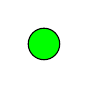
\begin{tikzpicture}
		\draw[fill=green] (0,0) circle (0.2cm);
	\end{tikzpicture}
}


\newpage 

\tikzstyle{block} = [draw, fill=blue!20,  rectangle, 
    minimum height=3em, minimum width=6em]
\tikzstyle{sum} = [draw, fill=blue!20, circle, node distance=1cm]
\tikzstyle{input} = [coordinate]
\tikzstyle{output} = [coordinate]
\tikzstyle{pinstyle} = [pin edge={to-, thin, black}]

% The block diagram code is probably more verbose than necessary
\begin{tikzpicture}[auto,  node distance=2cm, >=latex']

    % We start by placing the blocks
    \node [input, name=input] {};
    \node [sum, right of=input] (sum) {};
    \node [block, right of=sum] (controller) {\symbolA};
    
    % add label to controller
     \node[above of=controller] (ctrlabel)  [yshift=-0.75cm] {Controller};
     % add arrow from label to box
    \draw[->] (ctrlabel) -- (controller);
    
    % this is option 1: adding label on top
%    \node [block, right of=controller, pin={[pinstyle] above:Disturbances},
%            node distance=3cm] (system) {\symbolB};
	% this option 2: adding label on top
    \node [block, right of=controller, node distance=3cm] (system) {\symbolB};
    % add label "Disturbances" above system
    \node[above of=system] (syslabel) [yshift=-0.75cm] {Disturbances};
    \draw[->] (syslabel) -- (system);

    % We draw an edge between the controller and system block to 
    % calculate the coordinate "u". We need it to place the measurement block. 
    \draw [->] (controller) -- node[name=u] {$u$} (system);
    \node [output, right of=system] (output) {};
    \node [block, below of=u] (measurements) {\symbolC};
    
    % add label to "measurements" block
     \node[below of=measurements] (mealabel) [yshift=0.75cm] {Measurements};
    \draw[->] (mealabel) -- (measurements);
    

    % Once the nodes are placed, connecting them is easy. 
    \draw [draw,->] (input) -- node {$r$} (sum);
    \draw [->] (sum) -- node {$e$} (controller);
    \draw [->] (system) -- node [name=y] {$y$}(output);
    \draw [->] (y) |- (measurements);
%    \draw [->] (measurements) -| node[pos=0.99] {$-$} 
%        node [near end] {$y_m$} (sum);
    \draw [->] (measurements) -|  node  [near end] {$y_m$} (sum);
    \draw (sum) node [yshift=-7, xshift=-7]  {$-$};
\end{tikzpicture}



\newpage

\newpage 
% diagram 1111111111111111111111
\tikzstyle{block} = [draw, fill=blue!20,  rectangle, 
    minimum height=3em, minimum width=6em]
\tikzstyle{sum} = [draw, fill=blue!20, circle, node distance=1cm]
\tikzstyle{input} = [coordinate]
\tikzstyle{output} = [coordinate]
\tikzstyle{pinstyle} = [pin edge={to-, thin, black}]

% The block diagram code is probably more verbose than necessary
\begin{tikzpicture}[auto,  node distance=2cm, >=latex']

    % We start by placing the blocks
    \node [input = 0, name=input] {};
    \node [sum, right of=input] (sum) {};
    \node [block, right of=sum] (controller) {\symbolA};
    
    % add label to controller
     \node[above of=controller] (ctrlabel)  [yshift=-0.75cm] {Controller};
     % add arrow from label to box
    \draw[->] (ctrlabel) -- (controller);
    
    % this is option 1: adding label on top
%    \node [block, right of=controller, pin={[pinstyle] above:Disturbances},
%            node distance=3cm] (system) {\symbolB};
	% this option 2: adding label on top
    \node [block, right of=controller, node distance=3cm] (system) { System \symbolB};
    % add label "Disturbances" above system
    
    \draw[->] (syslabel) -- (system);

    % We draw an edge between the controller and system block to 
    % calculate the coordinate "u". We need it to place the measurement block. 
    \draw [->] (controller) -- node[name=u] {$u$} (system);
    \node [output, right of=system] (output) {};
    \node[above of=system] (syslabel) [yshift=-0.75cm] {Disturbances};
    

    

    % Once the nodes are placed, connecting them is easy. 
 
    \draw [->] (sum) -- node {$e$} (controller);
    \draw [->] (system) -- node [name=y] {$y$}(output);
 


\end{tikzpicture}


\newpage 
% diagram 22222222222222222222222222
\tikzstyle{block} = [draw, fill=blue!20,  rectangle, 
    minimum height=3em, minimum width=6em]
\tikzstyle{sum} = [draw, fill=blue!20, circle, node distance=1cm]
\tikzstyle{input} = [coordinate]
\tikzstyle{output} = [coordinate]
\tikzstyle{pinstyle} = [pin edge={to-, thin, black}]

% The block diagram code is probably more verbose than necessary
\begin{tikzpicture}[auto,  node distance=2cm, >=latex']

    % We start by placing the blocks
    \node [input = 0, name=input] {};
    \node [sum, right of=input] (sum) {};
    \node [block, right of=sum] (controller) {\symbolA};
    
    % add label to controller
     \node[above of=controller] (ctrlabel)  [yshift=-0.75cm] {Controller};
     % add arrow from label to box
    \draw[->] (ctrlabel) -- (controller);
    
    % this is option 1: adding label on top
%    \node [block, right of=controller, pin={[pinstyle] above:Disturbances},
%            node distance=3cm] (system) {\symbolB};
	% this option 2: adding label on top
    \node [block, right of=controller, node distance=3cm] (system) { System \symbolB};
    % add label "Disturbances" above system
    \node[above of=system] (syslabel) [yshift=-0.75cm] {Disturbances};
    \draw[->] (syslabel) -- (system);

    % We draw an edge between the controller and system block to 
    % calculate the coordinate "u". We need it to place the measurement block. 
    \draw [->] (controller) -- node[name=u] {$u$} (system);
    \node [output, right of=system] (output) {};
    \node [block, below of=u] (measurements) {\symbolC};
    
    % add label to "measurements" block
     \node[below of=measurements] (mealabel) [yshift=0.75cm] {Measurements};
    \draw[->] (mealabel) -- (measurements);
    

    % Once the nodes are placed, connecting them is easy. 
 
    \draw [->] (sum) -- node {$e$} (controller);
    \draw [->] (system) -- node [name=y] {$y$}(output);
    \draw [->] (y) |- (measurements);
%    \draw [->] (measurements) -| node[pos=0.99] {$-$} 
%        node [near end] {$y_m$} (sum);
    \draw [->] (measurements) -|  node  [near end] {$y_m$} (sum);
    \draw (sum) node [yshift=-7, xshift=-7]  {};
\end{tikzpicture}


\newpage


\begin{frame}
\frametitle{Automatics Flight Control }

\url{https://www.jkuse.com/home/jkhome/ph-d-thesis}

\url{https://www.ll.mit.edu/r-d/engineering/control-and-autonomous-systems-engineering}

\url{https://www.ll.mit.edu/about/facilities/autonomous-systems-development-facility}


\end{frame}
